
\chapter{Аналитический раздел}
\label{cha:analysis}

\section{Постановка задачи}

В соответствии с заданием на курсовую работу по курсу 
Операционные системы необходимо разработать загружаемый модуль ядра, предоставляющий пользователю 
возможность получения информации о виртуальной памяти процесса.
Также будет произведено исследование выделения виртуальной памяти
многопоточным приложениям на основе анализируемой программы, которая тоже будет реализованна
в данном курсовом проекте.% для демонстрации использования предоставленного по. 

Для решения задачи необходимо.

\begin{enumerate}
	\item Определить структуры, связанные с поставленной задачей.
	% TODO:
	\item Проанализировать и выбрать способ получения информации о виртуальной памяти процесса.
	\item Разработать алгоритм определения количества выделяемых процессу страниц по запросам на выделение памяти.
	\item Разработать структуру ПО.
	\item Реализовать ПО.
	\item Провести исследования выделения памяти.


	% \item Исследовать структуры, связанные с поставленной задачей.
	% \item Выполнить анализ и способ получения информации.
	% \item Разработать алгоритм.
	% \item Реализовать анализируемую программу.
	% \item Реализовать загружаемый модуль ядра, предоставляющий возможность анализа полей структур ядра, связанных с виртуальной памятью.
	% \item Привести пример анализа виртуальной памяти реализованной программы.   
\end{enumerate}

% TODO:
% метода лаба про форк карта (оптимизация форк) если не найду написать на почту 

% \section{Адресное пространство процесса}

% Ядро управляет памятью пользовательских программ.
% Эта память называется адресным пространством процесса (process address space) 
% и выделяется операционной системой каждому пользовательскому процессу.
% Операционная система Linux является системой с поддержкой виртуальной памяти,
% т.е. в ней выполняется виртуализация ресурсов памяти среди всех процессов в системе.
% Для каждого процесса создается иллюзия того, что он один использует всю физическую память в системе.
% Адресное пространство одного процесса может значительно превышать объем физической памяти компьютера.

% \subsection{Виртуальная адресное пространство}
\subsection{Анализ выделения памяти процессу}

Стали делить память на страницы. Можно выполнить программу, которая находится не целиком в памяти. 
Для этого нужно содержать части кода с которыми в текущий момент работает процессор.
Это воплотилось в понятие виртуальная память.

\textit{Виртуальная память} – память, размер которой превышает размер реального физического пространства.
Виртуальная память сама по себе ничего не хранит. 
Виртуальное адресное пространство — это абстракция, но оно определенным образом поставлено в соответствие физической памяти.

Загрузка частей программы в память выполняется по запросу. 
Т.е. соответствие части кода загружаемого по запросу, когда процессор обращается к этим частям кода.

\subsection{Таблица страниц}

Адресное пространство процесса и адресное пространство физической памяти делится на блоки равного размера. Блоки, на которые делится адресное пространство процесса называют страницами, а блоки на которые делится физическая память – кадрами, фреймами или блоками.

Виртуальный адрес состоит из двух частей:

\begin{itemize}
	\item p - номер страницы,
	\item d - смещение страницы.
\end{itemize}

На рис. \ref{fig:1} продемонстрировано отображение виртуальной памяти на физическую с помощью таблицы страниц.

\begin{figure}[ht!]
	\centering{
		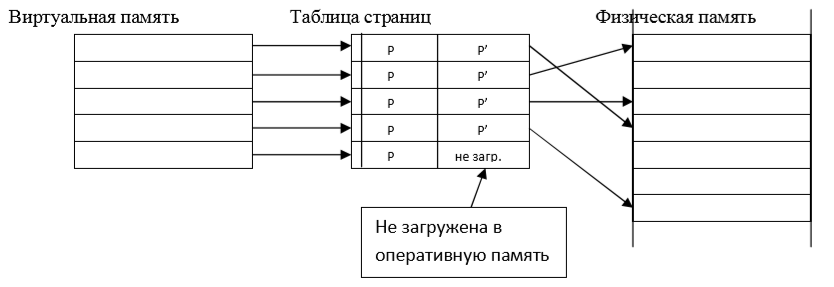
\includegraphics[width=0.8\textwidth]{img/1.png}
		\caption{Отображение виртуальной памяти на физическую с помощью таблицы страниц}
		\label{fig:1}}
\end{figure}

\newpage

% \subsection{Поле pgd}

С помощью таблиц страниц процессор осуществляет 
преобразование виртуального адреса в физический. 
У каждого процесса есть свой набор таблиц страниц.
Как только происходит переключение процесса (context switch), меняются и таблицы страниц. 
В Linux, указатель на таблицы страниц процесса хранится в поле pgd дескриптора памяти процесса. 
Каждой виртуальной странице соответствует одна запись в таблице страниц.

На рис. \ref{fig:2} показана 4-байтовая запись pgd.

\begin{figure}[ht!]
	\centering{
		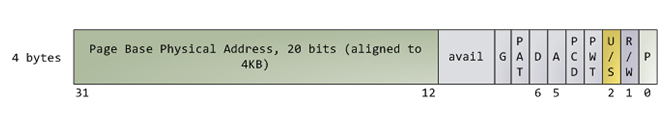
\includegraphics[width=1\textwidth]{img/2.jpg}
		\caption{4-байтовая запись pgd}
		\label{fig:2}}
\end{figure}

Флаг «P» говорит о том, находится ли страница в оперативной памяти или нет.
Когда данный флаг установлен в 0, доступ к соответствующей странице вызовет page fault.
Флаг «R/W» означает «запись/чтение»; если флаг не установлен, то к странице возможен доступ только на чтение.
Флаг «U/S» означает «пользователь/супервайзер»; если флаг не установлен, только код выполняющийся 
с уровнем привилегий 0 (т.е. ядро) может обратиться к данной странице.
Таким образом, данные флаги используются для того, чтобы реализовать концепцию адресного 
пространства доступного только на запись и пространства, которое доступно только для ядра.
Флаги «D» и «A» означают «dirty» и «accessed». «Dirty-страница» – эта та, в которую была недавно проведена запись, 
а «accessed»-страница – это страница, к которой было осуществлено обращение (чтение или запись). 
pgd хранит начальный физический адрес страницы в памяти.

При выполнении программы, которая находится не целиком в памяти, процесс потребует страницу, 
которой нет в оперативной памяти - возникнет исключение (страничная неудача - исправимое исключение), 
которое будет обработано в режиме ядра. В результате менеджер памяти попытается загрузить страницу 
в свободную память, а процесс на это время будет заблокирован. По завершении работы менеджера памяти страница
будет загружена и процесс будет продолжать выполнятся с той команды, на которой возникло исключение. 
Если свободная страница в физической памяти отсутствует, то менеджер памяти должен выбрать страницу для замещения.

Процесс может обращаться только к разрешенным областям памяти. 
Каждой области памяти назначаются определенные права доступа, такие как чтение, запись 
или выполнение, которые процесс должен неукоснительно соблюдать. 
Если процесс обращается по адресу, который не относится к разрешенной области памяти, 
или если доступ к разрешенной области памяти выполняется некорректным образом, ядро уничтожает такой
процесс с сообщением «Segmentation Fault» (Ошибка сегментации).

В областях памяти может содержаться вся нужная процессу информация, такая как:

\begin{itemize}
	\item машинный код, загруженный из исполняемого файла в область памяти процесса, которая называется сегментом кода (text section);
	\item инициализированные переменные, загруженные из исполняемого файла в область памяти процесса, которая называется сегментом данных (data section);
	\item страницы памяти, заполненные нулями, в которых содержатся неинициализированные глобальные переменные программы. Эта область памяти называется сегментом bss 1 (bss section);
	\item страницы памяти, заполненные нулями, в которых находится пользовательский стек процесса;
	\item дополнительные сегменты кода, данных и BSS для каждой совместно используемой библиотеки, такой как библиотека libc и динамический компоновщик, которые загружаются в адресное пространство процесса.
\end{itemize}

\section{Структуры ядра}

\subsection{Структура task\_struct}

Список процессов хранится в ядре в виде циклического двухсвязного списка, 
который называется списком задач (task list). 
Каждый элемент этого списка описывает один
запущенный процесс и называется дескриптором процесса. Дескриптор процесса имеет
тип task\_struct, структура которого описана в файле <linux/sched.h>. 
Дескриптор процесса содержит всю информацию об определенном процессе.
В дескрипторе процесса содержатся данные, которые описывают выполняющуюся
программу, — открытые файлы, адресное пространство процесса, сигналы, ожидающие
обработки, состояние процесса и многое другое (рис. \ref{fig:3}). 
На листинге 1.1 представлена часть структуры task\_struct.

\begin{figure}[ht!]
	\centering{
		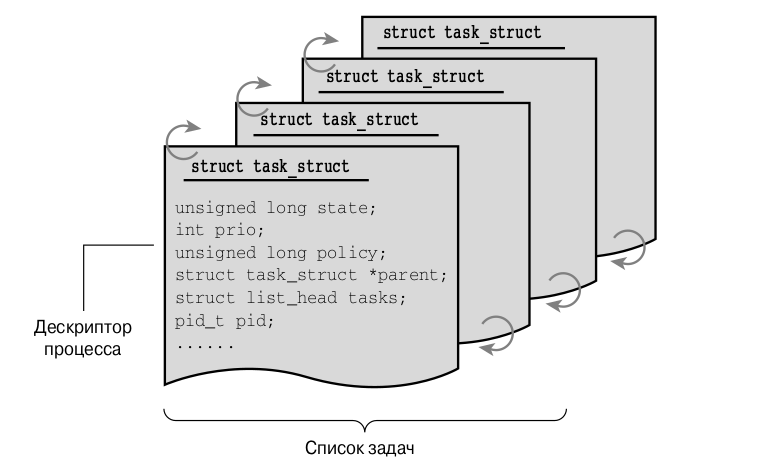
\includegraphics[width=1\textwidth]{img/3.png}
		\caption{Дескриптор процесса и список задач}
		\label{fig:3}}
\end{figure}

\newpage

\begin{lstlisting}[language=c, label=some-code, caption=Структура task\_struct]
struct task_struct {	
	void				*stack;
	refcount_t			usage;
	unsigned int			flags;
	unsigned int			ptrace;
	struct task_struct		*last_wakee;

	...

	unsigned int			policy;

	struct list_head		tasks;

	struct mm_struct		*mm;
	struct mm_struct		*active_mm;

	/* Per-thread vma caching: */
	struct vmacache			vmacache;

	int				exit_state;
	int				exit_code;
	int				exit_signal;

	pid_t				pid;
	pid_t				tgid;


	/* Real parent process: */
	struct task_struct __rcu	*real_parent;

	/* Recipient of SIGCHLD, wait4() reports: */
	struct task_struct __rcu	*parent;

	/*
	* Children/sibling form the list of natural children:
	*/
	struct list_head		children;
	struct list_head		sibling;
	struct task_struct		*group_leader;

	/* Filesystem information: */
	struct fs_struct		*fs;

	/* Open file information: */
	struct files_struct		*files;

	/* Namespaces: */
	struct nsproxy			*nsproxy;

	/* Signal handlers: */
	struct signal_struct		*signal;
	struct sighand_struct		*sighand;
	sigset_t			blocked;
	sigset_t			real_blocked;

	/* VM state: */
	struct reclaim_state		*reclaim_state;

	struct backing_dev_info		*backing_dev_info;

	struct io_context		*io_context;
	
	...	

};
\end{lstlisting}

\subsection{Структура mm\_struct.}

Адресное пространство процесса представляется в ядре в виде структуры данных, 
которая называется дескриптором памяти (memory descriptor). 
В этой структуре содержится вся информация, относящаяся к адресному пространству процесса. 
Дескриптор памяти представляется с помощью структуры mm\_struct,
которая определена в файле <linux/mm\_types.h>. 
Указатель на данную структуру содерержится в поле mm структуры task\_struct.  
Структура вместе с поясняющими комментариями по каждому полю приведена на листинге 1.2

\begin{lstlisting}[language=c, label=some-code, caption=Структура mm\_struct]
struct mm_struct {
	struct vm_area_struct *mmap; 
	/* Список областей памяти */
	struct rb_root mm_rb; 
	/* Красно-черное дерево областей памяти */
	struct vm_area_struct *mmap_cache;
	/* Последняя использованная область памяти */
	unsigned long free_area_cache; 
	/* Первый незанятый участок адресного пространства */
	pgd_t *pgd;
	/* Глобальный каталог страниц */
	atomic_t mm_users; 
	/* Счетчик использования адресного пространства */
	atomic_t mm_count; 
	/* Основной счетчик использования */
	int map_count; 
	/* Количество областей памяти */
	struct rw_semaphore mmap_sem; 
	/* Семафор для областей памяти */
	spinlock_t page_table_lock; 
	/* Спин-блокировка таблиц страниц */
	struct list_head mmlist;
	/* Список всех структур mm_struct */
	unsigned long start_code;
	/* Начальный адрес сегмента кода */
	unsigned long end_code;
	/* Конечный адрес сегмента кода */
	unsigned long start_data;
	/* Начальный адрес сегмента данных */
	unsigned long end_data;
	/* Конечный адрес сегмента данных */
	unsigned long start_brk;
	/* Начальный адрес сегмента "кучи" */
	unsigned long brk;
	/* Конечный адрес сегмента "кучи" */
	unsigned long start_stack;
	/* Начало стека процесса */
	unsigned long arg_start; 
	/* Начальный адрес области аргументов */
	unsigned long arg_end;
	/* Конечный адрес области аргументов */
	unsigned long env_start; 
	/* Начальный адрес области переменных среды */
	unsigned long env_end;
	/* Конечный адрес области переменных среды */
	unsigned long rss;
	/* rss - Количество распределенных физических страниц памяти */
	unsigned long total_vm; 
	/* total_vm - Общее количество страниц памяти */
	unsigned long locked_vm; 
	/* Количество заблокированных страниц памяти */
	unsigned long saved_auxv[AT_VECTOR_SIZE]; 
	/* Сохраненный вектор auxv */
	cpumask_t cpu_vm_mask;
	/* Маска отложенного переключения буфера TLB */
	mm_context_t context; 
	/* Данные, специфичные для аппаратной платформы */
	unsigned long  flags;
	/* Флаги состояния */
	int core_waiters;
	/* количество потоков, ожидающих создания файла дампа */
	struct core_state *core_state; 
	/* Поддержка дампа */
	spinlock_t ioctx_lock; 
	/* Блокировка списка асинхронного ввода-вывода (AIO) */
	struct hlist_head ioctx_list; 
	/* Список асинхронного ввода-вывода (AIO) */
};
\end{lstlisting}

В поле mm\_users хранится количество процессов, в которых используется данное
адресное пространство. Например, если одно и то же адресное пространство 
используется в двух потоках, значение поля mm\_users равно 2.

В полях mmap и mm\_rb хранятся ссылки на две различные структуры данных, 
содержащие одну и ту же информацию: информацию обо всех областях памяти в 
соответствующем адресном пространстве. В первой структуре эта информация 
хранится в виде связанного списка, а во второй — в виде красно-черного дерева. 
Поскольку красно-черное дерево — это разновидность двоичного дерева, 
то, как и для всех типов двоичных деревьев,
количество операций поиска заданного элемента в нем подчиняется закону O(log(n)).

Все структуры mm\_struct объединены в двухсвязный список с помощью полей mmlist.

\subsection{Структура vm\_area\_struct}

Области памяти (memory areas) представляются с помощью структуры 
vm\_area\_struct, которая определена в файле <linux/mm\_types.h>.

Структура vm\_area\_struct используется для описания одной непрерывной 
области памяти в данном адресном пространстве. В ядре каждая область памяти считается
уникальным объектом. Для каждой области памяти определены некоторые общие 
свойства, такие как права доступа и набор соответствующих операций. Таким образом, 
каждая структура VMA может представлять различный тип области памяти, например 
файлы, отображаемые в память, или стек пользовательского приложения.
Структура vm\_area\_struct приведена на листинге 1.3.

\begin{lstlisting}[language=c, label=some-code, caption=Структура vm\_area\_struct]
struct vm_area_struct {
	struct mm_struct *vm_mm;
	/* Соответствующая структура mm_struct */
	unsigned long vm_start;/* Начало диапазона адресов (включительно) */
	unsigned long vm_end; /* Конец диапазона адресов (исключая) */
	struct vm_area_struct *vm_next; /* Список областей VMA */
	pgprot_t vm_page_prot; /* Права доступа */
	unsigned long vm_flags;/* Флаги */
	struct rb_node vm_rb; /* Узел текущей области VMA в дереве */
	union {
		/* Связь с address_space->i_mmap или i_mmap_nonlinear */
		struct {
			struct list_head list;
			void *parent;
			struct vm_area_struct *head;
		} vm_set;

		struct prio_tree_node prio_tree_node;
	} shared;
	struct list_head anon_vma_node; /* Элемент анонимной области */
	struct anon_vma *anon_vma; /* Объект анонимной VMA */
	struct vm_operations_struct *vm_ops; /* Связанные операции */
	unsigned long vm_pgoff; /* Смещение в файле */
	struct file *vm_file; /* Отображенный файл (если есть) */
	void *vm_private_data; /* Частные данные */
};
\end{lstlisting}

\subsection{Взаимосвязь приведенных структур}

Взаимосвязь приведенных структур продемонстрирована на рис. \ref{fig:4}

\begin{figure}[ht!]
	\centering{
		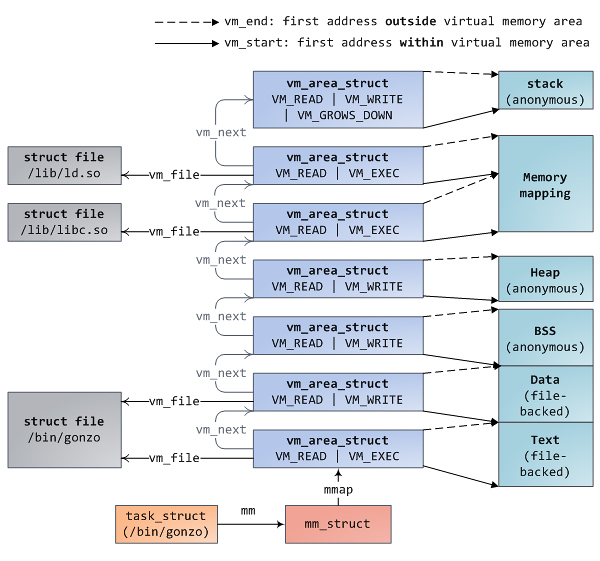
\includegraphics[width=0.7\textwidth]{img/4.jpg}
		\caption{Взаимосвязь приведенных структур}
		\label{fig:4}}
\end{figure}

\newpage

\section{Прерывания}

Прерывания делятся на:

\begin{itemize}
	\item исключения (деление на ноль, переполнение стека), синхронные;
	\item системные вызовы (программные) - вызываются с помощью соответствующей команды из программы (int 21h), синхронные;
	\item аппаратные прерывания (прерывания от системного таймера, клавиатуры), асинхронные. 
\end{itemize}

Прерывания делятся на 2 группы:

\begin{itemize}
	\item быстрые;
	\item медленные. 
\end{itemize}

Для того чтобы сократить время обработки медленных прерываний, они делятся на 2 части:

\begin{itemize}
	\item top half, верхняя половина, запускается в результате получения процессором сигнала прерывания;
	\item bottom half, нижняя половина, отложенные вызовы.
\end{itemize}

Существует несколько способов реализации “нижней половины“
обработчика: 
\begin{itemize}
	\item softirq;
	\item тасклет (tasklet);
	\item очереди работ (workqueue).
\end{itemize}
\subsection{Обработчики аппаратных прерываний}


// TODO: total\_vm  это не физич у тебя написано физи где-то
TODO:  Написать про то, что я написала обработчика  про то что из структур достаю информацию во время
выпорлнения в очереди. 

Обработчик прерывания должен выполнять минимальный объем действий и завершаться как можно быстрее.
Обычно такой обработчик прерывания сохраняет данные, поступившие от внешнего устройства, в буфере ядра. 
Но для того чтобы обработать прерывания полностью, обработчик аппаратного прерывания должен 
инициализировать постановку в очередь на выполнение отложенное действие.

\subsection{Очереди работ}

Очереди работ являются обобщенным механизмом отложенного выполнения, в котором 
функция обработчика, реализующая соответствующие действия, может блокироваться.

struct workqueue\_struct - описывает очередь работ.

\begin{lstlisting}[language=c, label=some-code, caption=Структура workqueue\_struct]
struct workqueue_struct {
	struct list_head    pwqs;        /* WR: all pwqs of this wq */
	struct list_head    list;        /* PR: list of all workqueues */
	...
	struct pool_workqueue    *dfl_pwq;    /* PW: only for unbound wqs */
	...
	struct pool_workqueue __percpu *cpu_pwqs; /* I: per-cpu pwqs */
	...
	};
\end{lstlisting}

struct work\_struct - описывает работу (обработчик нижней половины).

\begin{lstlisting}[language=c, label=some-code, caption=Структура workqueue\_struct]
struct work_struct {
	atomic_long_t data;
	struct list_head entry;
	work_func_t func;
	...
};
\end{lstlisting}

Работа может инициализироваться 2-мя способами:

\begin{itemize}
	\item статически;
	\item динамически.
\end{itemize}

При статической инициализации используется макрос:

\begin{lstlisting}[language=c, label=some-code, caption=статическая инициализация]
	DECLARE_WORK(name, void (*func)(void *));
\end{lstlisting}

где: name – имя структуры work\_struct, func – функция, которая вызывается из workqueue – обработчик нижней половины.

При динамической инициализации используются макросы:

\begin{lstlisting}[language=c, label=some-code, caption=динамическая инициализация]
	INIT_WORK(sruct work_struct *work, void (*func)(void),void *data);
\end{lstlisting}

После того, как будет инициализирована структура для объекта work, следующим шагом будет помещение этой структуры в очередь работ. 
Это можно сделать несколькими способами. 
Во-первых, можно добавить работу (объект work) в очередь работ с помощью функции queue\_work (которая назначает работу текущему процессору). 
Во-вторых, можно с помощью функции queue\_work\_on указать процессор, на котором будет выполняться обработчик.

\section{Вывод}

Были рассмотрены основополагающие материалы, которые в дальнейшем потребуются при реализации 
загружаемого модуля ядра.



